\documentclass[12pt,letterpaper]{hmcpset}
\usepackage[margin=1in]{geometry}
\usepackage{graphicx}
\usepackage{zach}
\usepackage{lmodern}
\usepackage{tikz}
\usepackage{algpseudocode}

% info for header block in upper right hand corner
\name{Zachary Seymour}
\class{CS 575}
\assignment{Theory Assignment 4}
\duedate{October 29, 2013}

\newcommand{\recur}[3]{T(n)=#1T(\frac{n}{#2})+#3}

\begin{document}

\problemlist{}

\begin{problem}[1]
Use the Master Theorem to solve the recurrences
\end{problem}

\begin{problem}[1a]
$\recur{4}{2}{n^3}$
\end{problem}

\begin{solution}
We have $\log_b a = \log_2 4 = 2$ and $f(n) = n^3$.  So, $\frac{n^3}{n^2} = n = \BigOmega{n^1}$, which is Case 3.  So $T(n) = \BigTheta{n^3}$.
\end{solution}

\begin{problem}[1b]
$\recur{2}{2}{n\lg^2 n}$
\end{problem}

\begin{solution}
We have $\log_b a = \log_2 2 = 1$ and $f(n) = n\lg^2 n$.  So, $\frac{n\lg^2 n}{n} = \lg^2 n = \BigTheta{\lg^2 n}$, which is Case 2.  So $T(n) = \BigTheta{n\lg^3 n}$.
\end{solution}

\begin{problem}[1c]
$\recur{3}{4}{n}$
\end{problem}

\begin{solution}
We have $\log_b a = \log_4 3$ and $f(n) = n$.  So, $\frac{n}{n^{\log_4 3}} = n^{1-\log_4 3} = \BigOmega{n^{1-\log_4 3}}$, which is Case 3.  So $T(n) = \BigTheta{n}$.
\end{solution}

\begin{problem}[1d]
$\recur{2}{4}{n\lg n}$
\end{problem}

\begin{solution}
We have $\log_b a = \log_4 2 = \frac{1}{2}$ and $f(n) = n\lg n$.  So, $\frac{n\lg n}{\sqrt{n}} = \sqrt{n} \lg n = \BigOmega{n}$, which is Case 3.  So $T(n) = \BigTheta{n\lg n}$.
\end{solution}

\begin{problem}[1e]
$\recur{4}{2}{n^2}$
\end{problem}

\begin{solution}
We have $\log_b a = \log_2 4 = 2$ and $f(n) = n^2$.  So, $\frac{n^2}{n^2} = 1 = \BigOmega{\lg^0 n}$, which is Case 2.  So $T(n) = \BigTheta{n^2 \lg n}$.
\end{solution}

\begin{problem}[1f]
$\recur{4}{2}{n^3}$
\end{problem}

\begin{solution}
We have $\log_b a = \log_2 4 = 2$ and $f(n) = n^3$.  So, $\frac{n^3}{n^2} = n = \BigOmega{n}$, which is Case 3.  So $T(n) = \BigTheta{n^3}$.
\end{solution}

\begin{problem}[2]
Use substitution to show that $T(n) = T(\frac{n}{2}) + T(\frac{n}{4}) + T(\frac{n}{9})$ belongs to $\BigTheta{n}$.
\end{problem}

\begin{solution}
We will guess an upper bound of $kn - b$.  We need to show that $T(n) \leq kn-b$ for all $n$.  Our base case is $n=1$.  We'll assume $T(1) = 1$.  So we have $1 = T(1) \leq k - b$, which holds as long as $k \geq b + 1$.  Now, we will assume this holds for $\frac{n}{2}$, $\frac{n}{4}$, and $\frac{n}{9}$.
\begin{align*}
T(n) &= T(\frac{n}{2}) + T(\frac{n}{4}) + T(\frac{n}{9}) \\
{} &= \frac{kn}{2} + \frac{kn}{4} + \frac{kn}{9} -3b \\
{} &= \frac{31kn}{36} - 3b \\
{} &\leq kn - b
\end{align*}
Thus, $T(n) = T(\frac{n}{2}) + T(\frac{n}{4}) + T(\frac{n}{9})$ belongs to $\BigTheta{n}$.
\end{solution}

\begin{problem}[3]
\[
T(n) =
\begin{cases}
\BigTheta{1} &\mbox{for } n \leq 1\\
T(\frac{n}{4}) + T(\frac{3n}{4}) &\mbox{otherwise}
\end{cases}
\]
\end{problem}

\begin{problem}[3a]
Show using the recursion tree method that $T(n) = \BigTheta{n\lg n}$ is a good guess.
\end{problem}

\begin{solution}
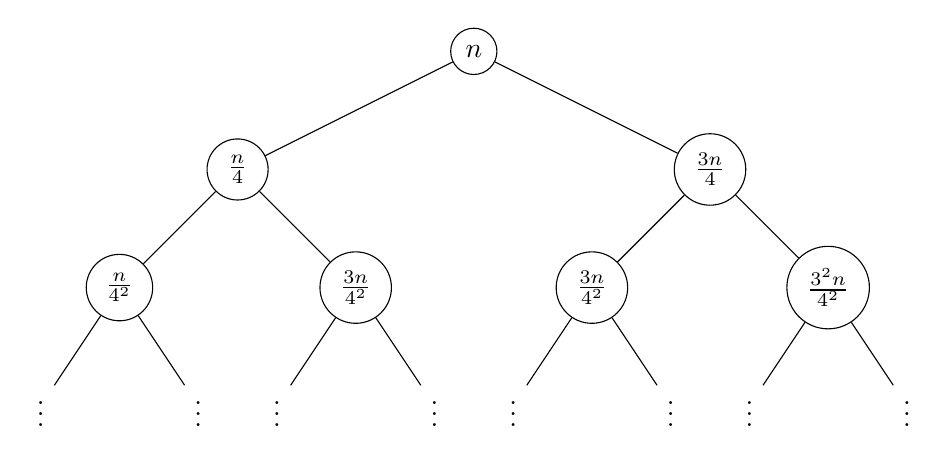
\begin{tikzpicture}[level/.style={sibling distance=60mm/#1}]
\node [circle,draw] (z){$n$}
  child {node [circle,draw] (a) {$\frac{n}{4}$}
    child {node [circle,draw] (b) {$\frac{n}{4^2}$}
      child {node {$\vdots$}} 
      child {node {$\vdots$}}
    }
    child {node [circle,draw] (g) {$\frac{3n}{4^2}$}
      child {node {$\vdots$}}
      child {node {$\vdots$}}
    }
  }
  child {node [circle,draw] (j) {$\frac{3n}{4}$}
    child {node [circle,draw] (k) {$\frac{3n}{4^2}$}
      child {node {$\vdots$}}
      child {node {$\vdots$}}
    }
  child {node [circle,draw] (l) {$\frac{3^2n}{4^2}$}
    child {node {$\vdots$}}
    child {node (c){$\vdots$}}
  }
};


\end{tikzpicture}

The two branches receive unequal portions of the work, with the rightmost branch being the longest, having length $\log_{4/3} n$.  Thus, our guess is $\BigTheta{n\lg n}$.
\end{solution}

\begin{problem}[3b]
Prove that $T(n) = \BigTheta{n\lg n}$ using the substitution method.
\end{problem}

\begin{solution}
\begin{proof}
We will guess an upper bound of $kn\lg bn$.  So, we need to show $T(n) \leq kn\lg bn$ for all $n$.  Our base case is $n = 1$.  We have $T(1) = \BigTheta{1} \leq k\cdot 1 \cdot \lg b =\lg b$.  Now, we will assume it holds for $\frac{n}{4}$ and $\frac{3n}{4}$.
\begin{align*}
T(n) &= T(\frac{n}{4}) + T(\frac{3n}{4}) \\
{} &= \frac{n}{4} \lg\left(b\frac{n}{4}\right) + \frac{3n}{4} \lg\left(b\frac{3n}{4}\right) \\
{} &= n \lg (\frac{3^{3/4}}{4}b n)\\
{} &\leq kn\lg bn
\end{align*}
\end{proof}
\end{solution}

\begin{problem}[Extra Credit]
Assume a MinHeap.  Assume that each record contains a key $k$ and data $d$.  Modify the \code{insert} and \code{deleteMin} procedure of a minheap so that the function \code{location(d)} (the index in the heap) takes only $\BigTheta{1}$ time.  Assume that $d$ is an integer between 0 and $n$.
\end{problem}

\begin{solution}
The only way I can really think to get constant time complexity is to use another array alongside the array storing the heap, where the indices, from 0 to $n$, are the data values.
\begin{algorithmic}
\Function{insert}{v}
\State last = last + 1
\State bt[last] $\leftarrow$ v
\State index = percolate(last)
\Comment{We would need percolate to return the true index.}
\State indices[v.d] $\leftarrow$ index
\EndFunction
\end{algorithmic}

\begin{algorithmic}
\Function{deleteMin}{}
\State minKeyItem = bt[root]
\State swap(root, last)
\State indices[minKeyItem.d] = NULL
\State last = last - 1
\If{last $> 0$}
\State siftDown(root)
\EndIf
\State \Return minKeyItem
\EndFunction
\end{algorithmic}
\end{solution}
\end{document}
